\documentclass{article}
\usepackage[utf8]{inputenc}
\usepackage{graphicx, float}
\usepackage{hyperref}
\usepackage{listings}
\usepackage{longtable}
\usepackage{multirow}
\usepackage{xcolor}
\usepackage{amsmath}

\title{CSP362: Database Management Systems - Assignment 2}
\author{SAHIL - 2016UCS0008 \\ RAHUL NIRANIA - 2016UCS0015}
\date{March 25, 2019}

\begin{document}

\maketitle

\tableofcontents

\section{Introduction}
\large
In this assignment, we have to create design a database for \textbf{Hospital Management System} in \textit{mysql} for deployment at \textbf{IIT Jammu}. The details of various modules have been provided. The entities and relationships are described based on the modules. An ER diagram has been made.

\section{Entities and Relationships}
The color scheme followed to list the attributes is as follows: \\ \\
{\color{blue}blue} for \textbf{Primary Key}. \\ \\
{\color{red}red} for \textbf{Foreign Key}. \\ \\
\begin{itemize}
    \item The following entities are required:
        \begin{itemize}
            \item \textbf{Patient}
                \begin{itemize}
                    \item {\color{blue}patient\_id}
                    \item name
                    \item gender
                    \item dob
                    \item weight
                    \item admitted (yes/no)
                    \item mother\_name
                    \item contact\_no
                    \item address
                \end{itemize}
            \item \textbf{Doctor}
                \begin{itemize}
                    \item {\color{blue}doctor\_id}
                    \item dob
                    \item gender
                    \item department
                    \item qualification
                    \item contact\_no
                    \item address
                    \item email
                    \item salary
                \end{itemize}
            \item \textbf{Staff}
                \begin{itemize}
                    \item {\color{blue}staff\_id}
                    \item type (consultant, intern, nurse)
                    \item name
                    \item dob
                    \item gender
                    \item address
                    \item contact\_no
                    \item salary
                    \item qualification
                \end{itemize}
            \item \textbf{Ward}
                \begin{itemize}
                    \item {\color{blue}ward\_id}
                    \item no\_of\_beds
                    \item class
                    \item current\_status
                \end{itemize}
            \item \textbf{Bed}
                \begin{itemize}
                    \item {\color{blue}bed\_id}
                    \item {\color{red}ward\_id}
                    \item {\color{red}patient\_id}
                \end{itemize}
            \item \textbf{Inpatient}
                \begin{itemize}
                    \item {\color{blue}patient\_id}
                    \item {\color{red}bed\_id}
                    \item date\_of\_admission
                    \item date\_of\_discharge
                \end{itemize}
            \item \textbf{Lab Report}
                \begin{itemize}
                    \item {\color{blue}lab\_id}
                    \item {\color{blue}report\_id}
                    \item {\color{red}patient\_id}
                    \item {\color{red}doctor\_id}
                    \item date
                    \item test\_type
                    \item result
                    \item amount
                \end{itemize}
            \item \textbf{Stock}
                \begin{itemize}
                    \item {\color{blue}stock\_id}
                    \item name
                    \item price
                    \item description
                    \item quantity\_available
                    \item type (medicine, equipment)
                \end{itemize}
        \end{itemize}
    \item The following relationships are required:
        \begin{itemize}
            \item \textbf{Patient\_Equipment}
                \begin{itemize}
                    \item {\color{blue}patient\_id}
                    \item {\color{blue}equipment\_id}
                \end{itemize}
            \item \textbf{Patient\_Bill}
                \begin{itemize}
                    \item {\color{blue}patient\_id}
                    \item eq\_bill\_amount (equipment)
                    \item tr\_bill\_amount (treatment, includes lab)
                    \item to\_bill\_amount (total)
                \end{itemize}
            \item \textbf{Patient\_Staff}
                \begin{itemize}
                    \item {\color{blue}patient\_id}
                    \item {\color{blue}staff\_id}
                \end{itemize}
        \end{itemize}
\end{itemize}

\section{Normalizing the database upto BCNF}
\subsection{1NF} The database design is already in \textbf{first normal form} since there is no field which is multi-valued.
\subsection{2NF} It is already in \textbf{second normal form} as there is no partial dependency of any non-key attribute on any key attribute. This is because all entity tables have single attribute as key, and for the relationship tables, there are only two attributes which themselves are part of the key.
\subsection{3NF} 
There are no transitive dependencies so the database is in \textbf{3NF}.

\subsection{BCNF} 
It is in \textbf{BCNF} as for all functional dependencies $X \rightarrow A$, $X$ is a super key.

\section{ER Diagram:}
\begin{figure}[H]
    \vspace{0pt}
    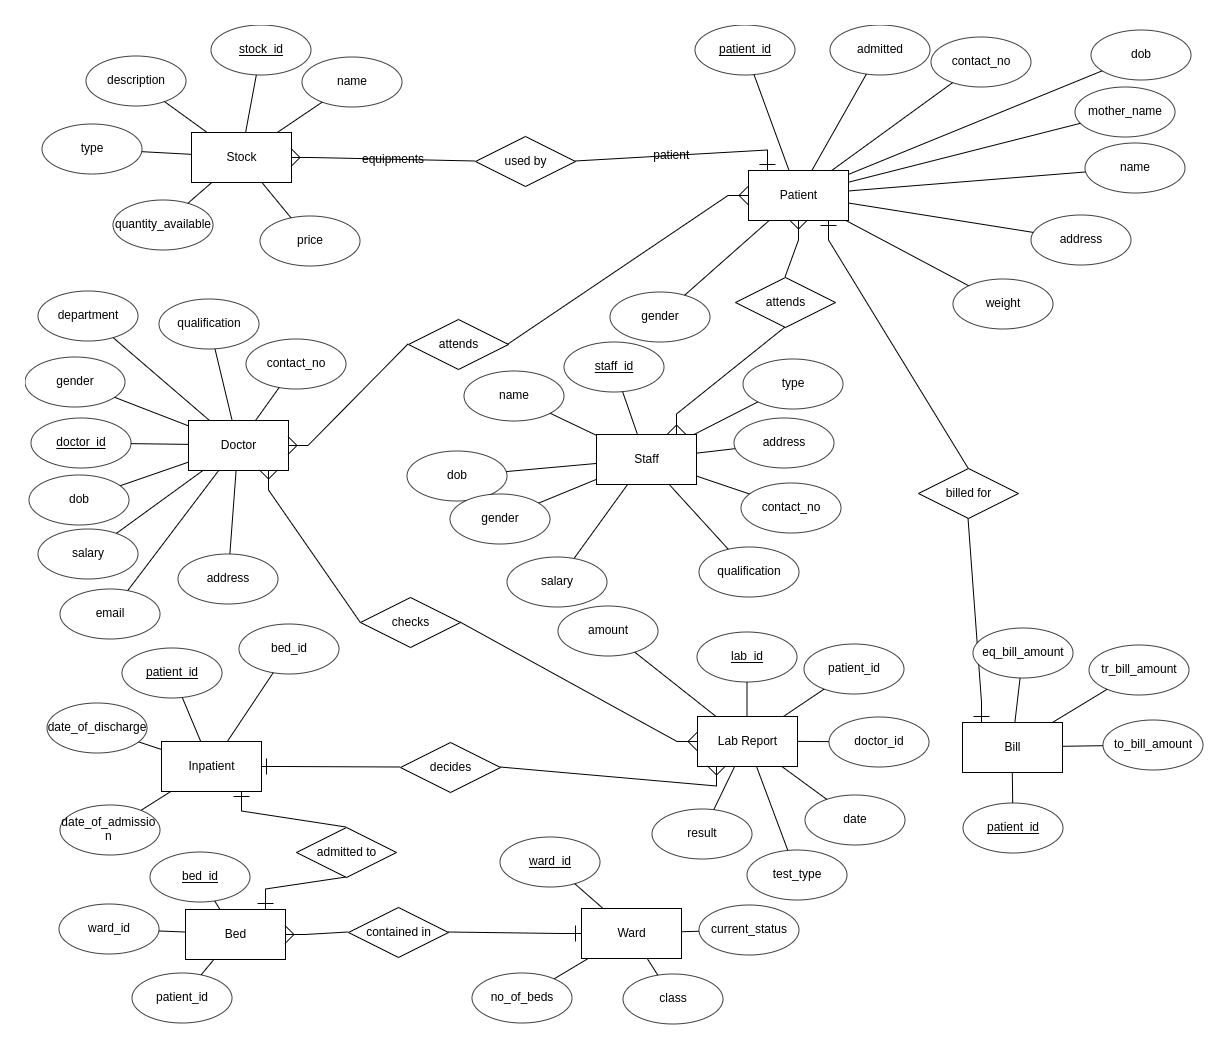
\includegraphics[width=450pt, keepaspectratio]{ER-Diagram.png}
\end{figure}
\end{document}
